\documentclass{article}
\title{\textbf{Setlist Manager}\\ \large{Official User Manual}}
\date{\vspace{-5ex}}
\usepackage[margin=1in]{geometry}
\usepackage{xcolor}
\usepackage{graphicx}
\graphicspath{{img/}}
\newcommand{\imgbox}[2]{\fcolorbox{darkgray}{white}{\includegraphics[width=#1px]{#2}}}
\newcommand{\cont}[1]{\noindent \fcolorbox{darkgray}{orange}{\begin{minipage}{200px} \section{#1} \end{minipage}}\\}
\newcommand{\scont}[1]{\noindent \fcolorbox{darkgray}{olive}{\begin{minipage}{200px} \subsection{#1} \end{minipage}}\\}

\renewcommand{\familydefault}{\sfdefault}
\begin{document}
\maketitle
\noindent \fcolorbox{darkgray}{lightgray}{\begin{minipage}{300px} \tableofcontents \end{minipage}}\\\\\\
\cont{Introduction}

Setlist Manager allows musicians to generate semi-random setlists for live music performance.\\\\
\cont{Catalog Management}

Select the "Catalog" tab 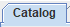
\includegraphics[width=20px]{tabCatalog.PNG} at the top of the window to manage your song catalog.\\
The song catalog is arranged alphabetically by composer, then title.\\

\scont{Open a Song Catalog}
\begin{enumerate}
\item In the "Catalog" tab, click the "Open Catalog" button 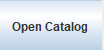
\includegraphics[width=30px]{openCatalog.PNG} located at the right side of the window.
\item Use the file browser to locate a song catalog file.\\\\ 
	\imgbox{175}{openBrowser.PNG}\\\\
	Song catalogs use a .setlist file extension.
\end{enumerate}

\scont{Add/Edit a Song}
\begin{enumerate}
	\item Click the "Edit" button next to an existing song in your catalog, or click the "Add Song" button on the right side of the window.\\\\
 	\imgbox{300}{addEdit.PNG}\\\\
	This will bring up a window where you will enter the song's data.\\\\
	\imgbox{200}{editSong.PNG}
	\item Enter the song title
	\item Enter the composer
	\item Enter the song's key
	\item Enter the song's genre.\\For songs that fit multiple genres, use a comma to in between each genre. 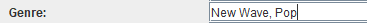
\includegraphics[width=110px]{genres.PNG}
	\item Enter the length of the song in seconds
	\item Enter the song's tempo in beats-per-minute(BPM)
	\item Enter an introduction time in seconds. The introduction time can be used to tell a story, explain a song's meaning, or introduce members of the band.
	\item The "Archive" checkbox prevents a song from being added to a setlist, but it will still be visible in the song catalog.
\end{enumerate}

\scont{Save/Export the Song Catalog}
\begin{enumerate}
	\item Click the "Export Catalog" button 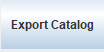
\includegraphics[width=30px]{exportCatalog.PNG} located at the right side of the window.
	\item Use the file browser to select a location and name for your song catalog file.\\\\
		\imgbox{175}{exportBrowser.PNG}
\end{enumerate}
\textcolor{red}{Note}: Any unsaved changes to the catalog will be lost when the program exits\\

\cont{Setlist Creation}\\
Select the "Setlist" tab 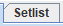
\includegraphics[width=20px]{tabSetlist.PNG} at the top of the window to create setlists.\\

\scont{Configure Setlist Length and Breaks}
\begin{enumerate}
	\item In the "Setlist" tab, click the "Setlist Settings" button 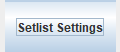
\includegraphics[width=30px]{setlistSettings.PNG} to open the Setlist Settings window.\\
		\imgbox{175}{setlistLength.PNG}
	\item Enter the set length in seconds.
	\item Enter the length of each break in seconds.
	\item Enter the number of breaks for the set.\\
	\textcolor{red}{Note}: Breaks are spaced evenly throughout the set.\\
	\item Click "OK" to save the settings.
\end{enumerate}

\scont{Filter Songs Individually}
\begin{enumerate}
	\item Locate the song in the "Catalog" tab, and click the "Edit" button.\\\\
		\imgbox{270}{archiveListing.PNG}\\\\
		The Edit Song window will appear.
	\item Click the "Archive" checkbox 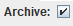
\includegraphics[width=25px]{archiveCheckbox.PNG} so the check mark appears. 
		\item Click "OK"
\end{enumerate}
The song will not be added to setlists until the check is removed.\\

\scont{Filter Songs by Genre}
\begin{enumerate}
	\item In the "Setlist" tab, click the "Setlist Settings" button 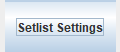
\includegraphics[width=30px]{setlistSettings.PNG} to open the Setlist Settings window.\\
	\item In the "Genre" field, enter any genre you wish to include in your setlist. \\\\
		\imgbox{200}{setlistGenres.PNG}
	\item Click OK
\end{enumerate}
		Any song that is not categorized in an included genre will not be added to a setlist.\\
		When the "Genre" field in Seltlist Settings is blank, all song genres will be available for a setlist.\\


\scont{Generate a Setlist}\\\\
\begin{minipage}{300px}
\begin{enumerate}
	\item Configure your setlist as described in the sections \textbf{Configure Setlist Length and Breaks}, \textbf{Filter Songs Individually}, and \textbf{Filter Songs by Genre}.
	\item In the "Setlist" tab, click the "Generate Setlist" button 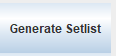
\includegraphics[width=30px]{generateSetlist.PNG} located at the right side of the window.\\
		The generated setlist will display in the main window.\\
		\textcolor{red}{Note}: You may see a warning, and generate an incomplete setlist if there are not enough songs in the catalog.\\\\
		\imgbox{200}{incomplete.PNG}
\end{enumerate}
\end{minipage}
\begin{minipage}{40px} \end{minipage}
\begin{minipage}{200px}     
\imgbox{200}{setlistExample.PNG}
\end{minipage}\\\\\\
\scont{Export/Share a Setlist}
\begin{enumerate}
	\item Generate a setlist as described in the \textbf{Generate a Setlist} section.
	\item In the "Setlist" tab, click the "Export Setlist" button 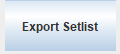
\includegraphics[width=30px]{exportSetlist.PNG}\\
		A file browser will appear.\\
		
		\imgbox{175}{saveSetlist.PNG}\\
	\item Select the file location, and name the file with a .html (formatted) or .txt (unformatted text) file extension.\\
		\item Click "Save"
\end{enumerate}

\end{document}
